%%%%%%%%%%%%%%%%%%%%%%%%%%%%%%%%%%%%%%%%%
% The Legrand Orange Book
% LaTeX Template
% Version 2.1.1 (14/2/16)
%
% This template has been downloaded from:
% http://www.LaTeXTemplates.com
%
% Original author:
% Mathias Legrand (legrand.mathias@gmail.com) with modifications by:
% Vel (vel@latextemplates.com)
%
% License:
% CC BY-NC-SA 3.0 (http://creativecommons.org/licenses/by-nc-sa/3.0/)
%
% Compiling this template:
% This template uses biber for its bibliography and makeindex for its index.
% When you first open the template, compile it from the command line with the 
% commands below to make sure your LaTeX distribution is configured correctly:
%
% 1) pdflatex main
% 2) makeindex main.idx -s StyleInd.ist
% 3) biber main
% 4) pdflatex main x 2
%
% After this, when you wish to update the bibliography/index use the appropriate
% command above and make sure to compile with pdflatex several times 
% afterwards to propagate your changes to the document.
%
% This template also uses a number of packages which may need to be
% updated to the newest versions for the template to compile. It is strongly
% recommended you update your LaTeX distribution if you have any
% compilation errors.
%
% Important note:
% Chapter heading images should have a 2:1 width:height ratio,
% e.g. 920px width and 460px height.
%
%%%%%%%%%%%%%%%%%%%%%%%%%%%%%%%%%%%%%%%%%

%----------------------------------------------------------------------------------------
%	PACKAGES AND OTHER DOCUMENT CONFIGURATIONS
%----------------------------------------------------------------------------------------

\documentclass[11pt,fleqn]{book} % Default font size and left-justified equations

%----------------------------------------------------------------------------------------

%%%%%%%%%%%%%%%%%%%%%%%%%%%%%%%%%%%%%%%%%
% The Legrand Orange Book
% Structural Definitions File
% Version 2.0 (9/2/15)
%
% Original author:
% Mathias Legrand (legrand.mathias@gmail.com) with modifications by:
% Vel (vel@latextemplates.com)
% 
% This file has been downloaded from:
% http://www.LaTeXTemplates.com
%
% License:
% CC BY-NC-SA 3.0 (http://creativecommons.org/licenses/by-nc-sa/3.0/)
%
%%%%%%%%%%%%%%%%%%%%%%%%%%%%%%%%%%%%%%%%%

%----------------------------------------------------------------------------------------
%	VARIOUS REQUIRED PACKAGES AND CONFIGURATIONS
%----------------------------------------------------------------------------------------

\usepackage[top=3cm,bottom=3cm,left=3cm,right=3cm,headsep=10pt,a4paper]{geometry} % Page margins

\usepackage{graphicx} % Required for including pictures
\graphicspath{{Pictures/}} % Specifies the directory where pictures are stored

\usepackage{tikz} % Required for drawing

\usepackage{pgfplots}
\pgfplotsset{width=10cm,compat=1.9}

\usepackage{circuitikz}

\usepackage{lipsum} % Inserts dummy text

\usepackage{tikz} % Required for drawing custom shapes

\usepackage[brazilian]{babel} % Pt-br language/hyphenation

\usepackage{enumitem} % Customize lists
\setlist{nolistsep} % Reduce spacing between bullet points and numbered lists

\usepackage{booktabs} % Required for nicer horizontal rules in tables

\usepackage{xcolor} % Required for specifying colors by name
\definecolor{ocre}{RGB}{0,104,179} % Define the orange color used for highlighting throughout the book

%----------------------------------------------------------------------------------------
%	FONTS
%----------------------------------------------------------------------------------------

\usepackage{avant} % Use the Avantgarde font for headings
%\usepackage{times} % Use the Times font for headings
\usepackage{mathptmx} % Use the Adobe Times Roman as the default text font together with math symbols from the Sym­bol, Chancery and Com­puter Modern fonts

\usepackage{microtype} % Slightly tweak font spacing for aesthetics
\usepackage[utf8]{inputenc} % Required for including letters with accents
\usepackage[T1]{fontenc} % Use 8-bit encoding that has 256 glyphs

%----------------------------------------------------------------------------------------
%	BIBLIOGRAPHY AND INDEX
%----------------------------------------------------------------------------------------

\usepackage[style=alphabetic,citestyle=numeric,sorting=nyt,sortcites=true,autopunct=true,babel=hyphen,hyperref=true,abbreviate=false,backref=true,backend=biber]{biblatex}
\addbibresource{bibliography.bib} % BibTeX bibliography file
\defbibheading{bibempty}{}

\usepackage{calc} % For simpler calculation - used for spacing the index letter headings correctly
\usepackage{makeidx} % Required to make an index
\makeindex % Tells LaTeX to create the files required for indexing

%----------------------------------------------------------------------------------------
%	MAIN TABLE OF CONTENTS
%----------------------------------------------------------------------------------------

\usepackage{titletoc} % Required for manipulating the table of contents

\contentsmargin{0cm} % Removes the default margin

% Part text styling
\titlecontents{part}[0cm]
{\addvspace{20pt}\centering\large\bfseries}
{}
{}
{}

% Chapter text styling
\titlecontents{chapter}[1.25cm] % Indentation
{\addvspace{12pt}\large\sffamily\bfseries} % Spacing and font options for chapters
{\color{ocre!60}\contentslabel[\Large\thecontentslabel]{1.25cm}\color{ocre}} % Chapter number
{\color{ocre}}  
{\color{ocre!60}\normalsize\;\titlerule*[.5pc]{.}\;\thecontentspage} % Page number

% Section text styling
\titlecontents{section}[1.25cm] % Indentation
{\addvspace{3pt}\sffamily\bfseries} % Spacing and font options for sections
{\contentslabel[\thecontentslabel]{1.25cm}} % Section number
{}
{\hfill\color{black}\thecontentspage} % Page number
[]

% Subsection text styling
\titlecontents{subsection}[1.25cm] % Indentation
{\addvspace{1pt}\sffamily\small} % Spacing and font options for subsections
{\contentslabel[\thecontentslabel]{1.25cm}} % Subsection number
{}
{\ \titlerule*[.5pc]{.}\;\thecontentspage} % Page number
[]

% List of figures
\titlecontents{figure}[0em]
{\addvspace{-5pt}\sffamily}
{\thecontentslabel\hspace*{1em}}
{}
{\ \titlerule*[.5pc]{.}\;\thecontentspage}
[]

% List of tables
\titlecontents{table}[0em]
{\addvspace{-5pt}\sffamily}
{\thecontentslabel\hspace*{1em}}
{}
{\ \titlerule*[.5pc]{.}\;\thecontentspage}
[]

%----------------------------------------------------------------------------------------
%	MINI TABLE OF CONTENTS IN PART HEADS
%----------------------------------------------------------------------------------------

% Chapter text styling
\titlecontents{lchapter}[0em] % Indenting
{\addvspace{15pt}\large\sffamily\bfseries} % Spacing and font options for chapters
{\color{ocre}\contentslabel[\Large\thecontentslabel]{1.25cm}\color{ocre}} % Chapter number
{}  
{\color{ocre}\normalsize\sffamily\bfseries\;\titlerule*[.5pc]{.}\;\thecontentspage} % Page number

% Section text styling
\titlecontents{lsection}[0em] % Indenting
{\sffamily\small} % Spacing and font options for sections
{\contentslabel[\thecontentslabel]{1.25cm}} % Section number
{}
{}

% Subsection text styling
\titlecontents{lsubsection}[.5em] % Indentation
{\normalfont\footnotesize\sffamily} % Font settings
{}
{}
{}

%----------------------------------------------------------------------------------------
%	PAGE HEADERS
%----------------------------------------------------------------------------------------

\usepackage{fancyhdr} % Required for header and footer configuration

\pagestyle{fancy}
\renewcommand{\chaptermark}[1]{\markboth{\sffamily\normalsize\bfseries\chaptername\ \thechapter.\ #1}{}} % Chapter text font settings
\renewcommand{\sectionmark}[1]{\markright{\sffamily\normalsize\thesection\hspace{5pt}#1}{}} % Section text font settings
\fancyhf{} \fancyhead[LE,RO]{\sffamily\normalsize\thepage} % Font setting for the page number in the header
\fancyhead[LO]{\rightmark} % Print the nearest section name on the left side of odd pages
\fancyhead[RE]{\leftmark} % Print the current chapter name on the right side of even pages
\renewcommand{\headrulewidth}{0.5pt} % Width of the rule under the header
\addtolength{\headheight}{2.5pt} % Increase the spacing around the header slightly
\renewcommand{\footrulewidth}{0pt} % Removes the rule in the footer
\fancypagestyle{plain}{\fancyhead{}\renewcommand{\headrulewidth}{0pt}} % Style for when a plain pagestyle is specified

% Removes the header from odd empty pages at the end of chapters
\makeatletter
\renewcommand{\cleardoublepage}{
\clearpage\ifodd\c@page\else
\hbox{}
\vspace*{\fill}
\thispagestyle{empty}
\newpage
\fi}

%----------------------------------------------------------------------------------------
%	THEOREM STYLES
%----------------------------------------------------------------------------------------

\usepackage{amsmath,amsfonts,amssymb,amsthm} % For math equations, theorems, symbols, etc

\newcommand{\intoo}[2]{\mathopen{]}#1\,;#2\mathclose{[}}
\newcommand{\ud}{\mathop{\mathrm{{}d}}\mathopen{}}
\newcommand{\intff}[2]{\mathopen{[}#1\,;#2\mathclose{]}}
\newtheorem{notation}{Notation}[chapter]

% Boxed/framed environments
\newtheoremstyle{ocrenumbox}% % Theorem style name
{0pt}% Space above
{0pt}% Space below
{\normalfont}% % Body font
{}% Indent amount
{\small\bf\sffamily\color{ocre}}% % Theorem head font
{\;}% Punctuation after theorem head
{0.25em}% Space after theorem head
{\small\sffamily\color{ocre}\thmname{#1}\nobreakspace\thmnumber{\@ifnotempty{#1}{}\@upn{#2}}% Theorem text (e.g. Theorem 2.1)
\thmnote{\nobreakspace\the\thm@notefont\sffamily\bfseries\color{black}---\nobreakspace#3.}} % Optional theorem note
\renewcommand{\qedsymbol}{$\blacksquare$}% Optional qed square

\newtheoremstyle{blacknumex}% Theorem style name
{5pt}% Space above
{5pt}% Space below
{\normalfont}% Body font
{} % Indent amount
{\small\bf\sffamily}% Theorem head font
{\;}% Punctuation after theorem head
{0.25em}% Space after theorem head
{\small\sffamily{\tiny\ensuremath{\blacksquare}}\nobreakspace\thmname{#1}\nobreakspace\thmnumber{\@ifnotempty{#1}{}\@upn{#2}}% Theorem text (e.g. Theorem 2.1)
\thmnote{\nobreakspace\the\thm@notefont\sffamily\bfseries---\nobreakspace#3.}}% Optional theorem note

\newtheoremstyle{blacknumbox} % Theorem style name
{0pt}% Space above
{0pt}% Space below
{\normalfont}% Body font
{}% Indent amount
{\small\bf\sffamily}% Theorem head font
{\;}% Punctuation after theorem head
{0.25em}% Space after theorem head
{\small\sffamily\thmname{#1}\nobreakspace\thmnumber{\@ifnotempty{#1}{}\@upn{#2}}% Theorem text (e.g. Theorem 2.1)
\thmnote{\nobreakspace\the\thm@notefont\sffamily\bfseries---\nobreakspace#3.}}% Optional theorem note

% Non-boxed/non-framed environments
\newtheoremstyle{ocrenum}% % Theorem style name
{5pt}% Space above
{5pt}% Space below
{\normalfont}% % Body font
{}% Indent amount
{\small\bf\sffamily\color{ocre}}% % Theorem head font
{\;}% Punctuation after theorem head
{0.25em}% Space after theorem head
{\small\sffamily\color{ocre}\thmname{#1}\nobreakspace\thmnumber{\@ifnotempty{#1}{}\@upn{#2}}% Theorem text (e.g. Theorem 2.1)
\thmnote{\nobreakspace\the\thm@notefont\sffamily\bfseries\color{black}---\nobreakspace#3.}} % Optional theorem note
\renewcommand{\qedsymbol}{$\blacksquare$}% Optional qed square
\makeatother

% Defines the theorem text style for each type of theorem to one of the three styles above
\newcounter{dummy} 
\numberwithin{dummy}{section}
\theoremstyle{ocrenumbox}
\newtheorem{theoremeT}[dummy]{Theorem}
\newtheorem{problem}{Problem}[chapter]
\newtheorem{exerciseT}{Exercise}[chapter]
\theoremstyle{blacknumex}
\newtheorem{exampleT}{Example}[chapter]
\theoremstyle{blacknumbox}
\newtheorem{vocabulary}{Vocabulary}[chapter]
\newtheorem{definitionT}{Definition}[section]
\newtheorem{corollaryT}[dummy]{Corollary}
\theoremstyle{ocrenum}
\newtheorem{proposition}[dummy]{Proposition}

%----------------------------------------------------------------------------------------
%	DEFINITION OF COLORED BOXES
%----------------------------------------------------------------------------------------

\RequirePackage[framemethod=default]{mdframed} % Required for creating the theorem, definition, exercise and corollary boxes

% Theorem box
\newmdenv[skipabove=7pt,
skipbelow=7pt,
backgroundcolor=black!5,
linecolor=ocre,
innerleftmargin=5pt,
innerrightmargin=5pt,
innertopmargin=5pt,
leftmargin=0cm,
rightmargin=0cm,
innerbottommargin=5pt]{tBox}

% Exercise box	  
\newmdenv[skipabove=7pt,
skipbelow=7pt,
rightline=false,
leftline=true,
topline=false,
bottomline=false,
backgroundcolor=ocre!10,
linecolor=ocre,
innerleftmargin=5pt,
innerrightmargin=5pt,
innertopmargin=5pt,
innerbottommargin=5pt,
leftmargin=0cm,
rightmargin=0cm,
linewidth=4pt]{eBox}	

% Definition box
\newmdenv[skipabove=7pt,
skipbelow=7pt,
rightline=false,
leftline=true,
topline=false,
bottomline=false,
linecolor=ocre,
innerleftmargin=5pt,
innerrightmargin=5pt,
innertopmargin=0pt,
leftmargin=0cm,
rightmargin=0cm,
linewidth=4pt,
innerbottommargin=0pt]{dBox}	

% Corollary box
\newmdenv[skipabove=7pt,
skipbelow=7pt,
rightline=false,
leftline=true,
topline=false,
bottomline=false,
linecolor=gray,
backgroundcolor=black!5,
innerleftmargin=5pt,
innerrightmargin=5pt,
innertopmargin=5pt,
leftmargin=0cm,
rightmargin=0cm,
linewidth=4pt,
innerbottommargin=5pt]{cBox}

% Creates an environment for each type of theorem and assigns it a theorem text style from the "Theorem Styles" section above and a colored box from above
\newenvironment{theorem}{\begin{tBox}\begin{theoremeT}}{\end{theoremeT}\end{tBox}}
\newenvironment{exercise}{\begin{eBox}\begin{exerciseT}}{\hfill{\color{ocre}\tiny\ensuremath{\blacksquare}}\end{exerciseT}\end{eBox}}				  
\newenvironment{definition}{\begin{dBox}\begin{definitionT}}{\end{definitionT}\end{dBox}}	
\newenvironment{example}{\begin{exampleT}}{\hfill{\tiny\ensuremath{\blacksquare}}\end{exampleT}}		
\newenvironment{corollary}{\begin{cBox}\begin{corollaryT}}{\end{corollaryT}\end{cBox}}	

%----------------------------------------------------------------------------------------
%	REMARK ENVIRONMENT
%----------------------------------------------------------------------------------------

\newenvironment{remark}{\par\vspace{10pt}\small % Vertical white space above the remark and smaller font size
\begin{list}{}{
\leftmargin=35pt % Indentation on the left
\rightmargin=25pt}\item\ignorespaces % Indentation on the right
\makebox[-2.5pt]{\begin{tikzpicture}[overlay]
\node[draw=ocre!60,line width=1pt,circle,fill=ocre!25,font=\sffamily\bfseries,inner sep=2pt,outer sep=0pt] at (-15pt,0pt){\textcolor{ocre}{R}};\end{tikzpicture}} % Orange R in a circle
\advance\baselineskip -1pt}{\end{list}\vskip5pt} % Tighter line spacing and white space after remark

%----------------------------------------------------------------------------------------
%	SECTION NUMBERING IN THE MARGIN
%----------------------------------------------------------------------------------------

\makeatletter
\renewcommand{\@seccntformat}[1]{\llap{\textcolor{ocre}{\csname the#1\endcsname}\hspace{1em}}}                    
\renewcommand{\section}{\@startsection{section}{1}{\z@}
{-4ex \@plus -1ex \@minus -.4ex}
{1ex \@plus.2ex }
{\normalfont\large\sffamily\bfseries}}
\renewcommand{\subsection}{\@startsection {subsection}{2}{\z@}
{-3ex \@plus -0.1ex \@minus -.4ex}
{0.5ex \@plus.2ex }
{\normalfont\sffamily\bfseries}}
\renewcommand{\subsubsection}{\@startsection {subsubsection}{3}{\z@}
{-2ex \@plus -0.1ex \@minus -.2ex}
{.2ex \@plus.2ex }
{\normalfont\small\sffamily\bfseries}}                        
\renewcommand\paragraph{\@startsection{paragraph}{4}{\z@}
{-2ex \@plus-.2ex \@minus .2ex}
{.1ex}
{\normalfont\small\sffamily\bfseries}}

%----------------------------------------------------------------------------------------
%	PART HEADINGS
%----------------------------------------------------------------------------------------

% numbered part in the table of contents
\newcommand{\@mypartnumtocformat}[2]{%
\setlength\fboxsep{0pt}%
\noindent\colorbox{ocre!20}{\strut\parbox[c][.7cm]{\ecart}{\color{ocre!70}\Large\sffamily\bfseries\centering#1}}\hskip\esp\colorbox{ocre!40}{\strut\parbox[c][.7cm]{\linewidth-\ecart-\esp}{\Large\sffamily\centering#2}}}%
%%%%%%%%%%%%%%%%%%%%%%%%%%%%%%%%%%
% unnumbered part in the table of contents
\newcommand{\@myparttocformat}[1]{%
\setlength\fboxsep{0pt}%
\noindent\colorbox{ocre!40}{\strut\parbox[c][.7cm]{\linewidth}{\Large\sffamily\centering#1}}}%
%%%%%%%%%%%%%%%%%%%%%%%%%%%%%%%%%%
\newlength\esp
\setlength\esp{4pt}
\newlength\ecart
\setlength\ecart{1.2cm-\esp}
\newcommand{\thepartimage}{}%
\newcommand{\partimage}[1]{\renewcommand{\thepartimage}{#1}}%
\def\@part[#1]#2{%
\ifnum \c@secnumdepth >-2\relax%
\refstepcounter{part}%
\addcontentsline{toc}{part}{\texorpdfstring{\protect\@mypartnumtocformat{\thepart}{#1}}{\partname~\thepart\ ---\ #1}}
\else%
\addcontentsline{toc}{part}{\texorpdfstring{\protect\@myparttocformat{#1}}{#1}}%
\fi%
\startcontents%
\markboth{}{}%
{\thispagestyle{empty}%
\begin{tikzpicture}[remember picture,overlay]%
\node at (current page.north west){\begin{tikzpicture}[remember picture,overlay]%	
\fill[ocre!20](0cm,0cm) rectangle (\paperwidth,-\paperheight);
\node[anchor=north] at (4cm,-3.25cm){\color{ocre!40}\fontsize{220}{100}\sffamily\bfseries\@Roman\c@part}; 
\node[anchor=south east] at (\paperwidth-1cm,-\paperheight+1cm){\parbox[t][][t]{8.5cm}{
\printcontents{l}{0}{\setcounter{tocdepth}{1}}%
}};
\node[anchor=north east] at (\paperwidth-1.5cm,-3.25cm){\parbox[t][][t]{15cm}{\strut\raggedleft\color{white}\fontsize{30}{30}\sffamily\bfseries#2}};
\end{tikzpicture}};
\end{tikzpicture}}%
\@endpart}
\def\@spart#1{%
\startcontents%
\phantomsection
{\thispagestyle{empty}%
\begin{tikzpicture}[remember picture,overlay]%
\node at (current page.north west){\begin{tikzpicture}[remember picture,overlay]%	
\fill[ocre!20](0cm,0cm) rectangle (\paperwidth,-\paperheight);
\node[anchor=north east] at (\paperwidth-1.5cm,-3.25cm){\parbox[t][][t]{15cm}{\strut\raggedleft\color{white}\fontsize{30}{30}\sffamily\bfseries#1}};
\end{tikzpicture}};
\end{tikzpicture}}
\addcontentsline{toc}{part}{\texorpdfstring{%
\setlength\fboxsep{0pt}%
\noindent\protect\colorbox{ocre!40}{\strut\protect\parbox[c][.7cm]{\linewidth}{\Large\sffamily\protect\centering #1\quad\mbox{}}}}{#1}}%
\@endpart}
\def\@endpart{\vfil\newpage
\if@twoside
\if@openright
\null
\thispagestyle{empty}%
\newpage
\fi
\fi
\if@tempswa
\twocolumn
\fi}

%----------------------------------------------------------------------------------------
%	CHAPTER HEADINGS
%----------------------------------------------------------------------------------------

% A switch to conditionally include a picture, implemented by  Christian Hupfer
\newif\ifusechapterimage
\usechapterimagetrue
\newcommand{\thechapterimage}{}%
\newcommand{\chapterimage}[1]{\ifusechapterimage\renewcommand{\thechapterimage}{#1}\fi}%
\def\@makechapterhead#1{%
{\parindent \z@ \raggedright \normalfont
\ifnum \c@secnumdepth >\m@ne
\if@mainmatter
\begin{tikzpicture}[remember picture,overlay]
\node at (current page.north west)
{\begin{tikzpicture}[remember picture,overlay]
\node[anchor=north west,inner sep=0pt] at (0,0) {\ifusechapterimage\includegraphics[width=\paperwidth]{\thechapterimage}\fi};
\draw[anchor=west] (\Gm@lmargin,-9cm) node [line width=2pt,rounded corners=15pt,draw=ocre,fill=white,fill opacity=0.5,inner sep=15pt]{\strut\makebox[22cm]{}};
\draw[anchor=west] (\Gm@lmargin+.3cm,-9cm) node {\huge\sffamily\bfseries\color{black}\thechapter. #1\strut};
\end{tikzpicture}};
\end{tikzpicture}
\else
\begin{tikzpicture}[remember picture,overlay]
\node at (current page.north west)
{\begin{tikzpicture}[remember picture,overlay]
\node[anchor=north west,inner sep=0pt] at (0,0) {\ifusechapterimage\includegraphics[width=\paperwidth]{\thechapterimage}\fi};
\draw[anchor=west] (\Gm@lmargin,-9cm) node [line width=2pt,rounded corners=15pt,draw=ocre,fill=white,fill opacity=0.5,inner sep=15pt]{\strut\makebox[22cm]{}};
\draw[anchor=west] (\Gm@lmargin+.3cm,-9cm) node {\huge\sffamily\bfseries\color{black}#1\strut};
\end{tikzpicture}};
\end{tikzpicture}
\fi\fi\par\vspace*{270\p@}}}

%-------------------------------------------

\def\@makeschapterhead#1{%
\begin{tikzpicture}[remember picture,overlay]
\node at (current page.north west)
{\begin{tikzpicture}[remember picture,overlay]
\node[anchor=north west,inner sep=0pt] at (0,0) {\ifusechapterimage\includegraphics[width=\paperwidth]{\thechapterimage}\fi};
\draw[anchor=west] (\Gm@lmargin,-9cm) node [line width=2pt,rounded corners=15pt,draw=ocre,fill=white,fill opacity=0.5,inner sep=15pt]{\strut\makebox[22cm]{}};
\draw[anchor=west] (\Gm@lmargin+.3cm,-9cm) node {\huge\sffamily\bfseries\color{black}#1\strut};
\end{tikzpicture}};
\end{tikzpicture}
\par\vspace*{270\p@}}
\makeatother

%----------------------------------------------------------------------------------------
%	HYPERLINKS IN THE DOCUMENTS
%----------------------------------------------------------------------------------------

\usepackage{hyperref}
\hypersetup{hidelinks,backref=true,pagebackref=true,hyperindex=true,colorlinks=false,breaklinks=true,urlcolor= ocre,bookmarks=true,bookmarksopen=false,pdftitle={Title},pdfauthor={Author}}
\usepackage{bookmark}
\bookmarksetup{
open,
numbered,
addtohook={%
\ifnum\bookmarkget{level}=0 % chapter
\bookmarksetup{bold}%
\fi
\ifnum\bookmarkget{level}=-1 % part
\bookmarksetup{color=ocre,bold}%
\fi
}
}
 % Insert the commands.tex file which contains the majority of the structure behind the template

\begin{document}

%----------------------------------------------------------------------------------------
%	TITLE PAGE
%----------------------------------------------------------------------------------------

\begingroup
\thispagestyle{empty}
\begin{tikzpicture}[remember picture,overlay]
\coordinate [below=12cm] (midpoint) at (current page.north);
\node at (current page.north west)
{\begin{tikzpicture}[remember picture,overlay]
\node[anchor=north west,inner sep=0pt] at (0,0) {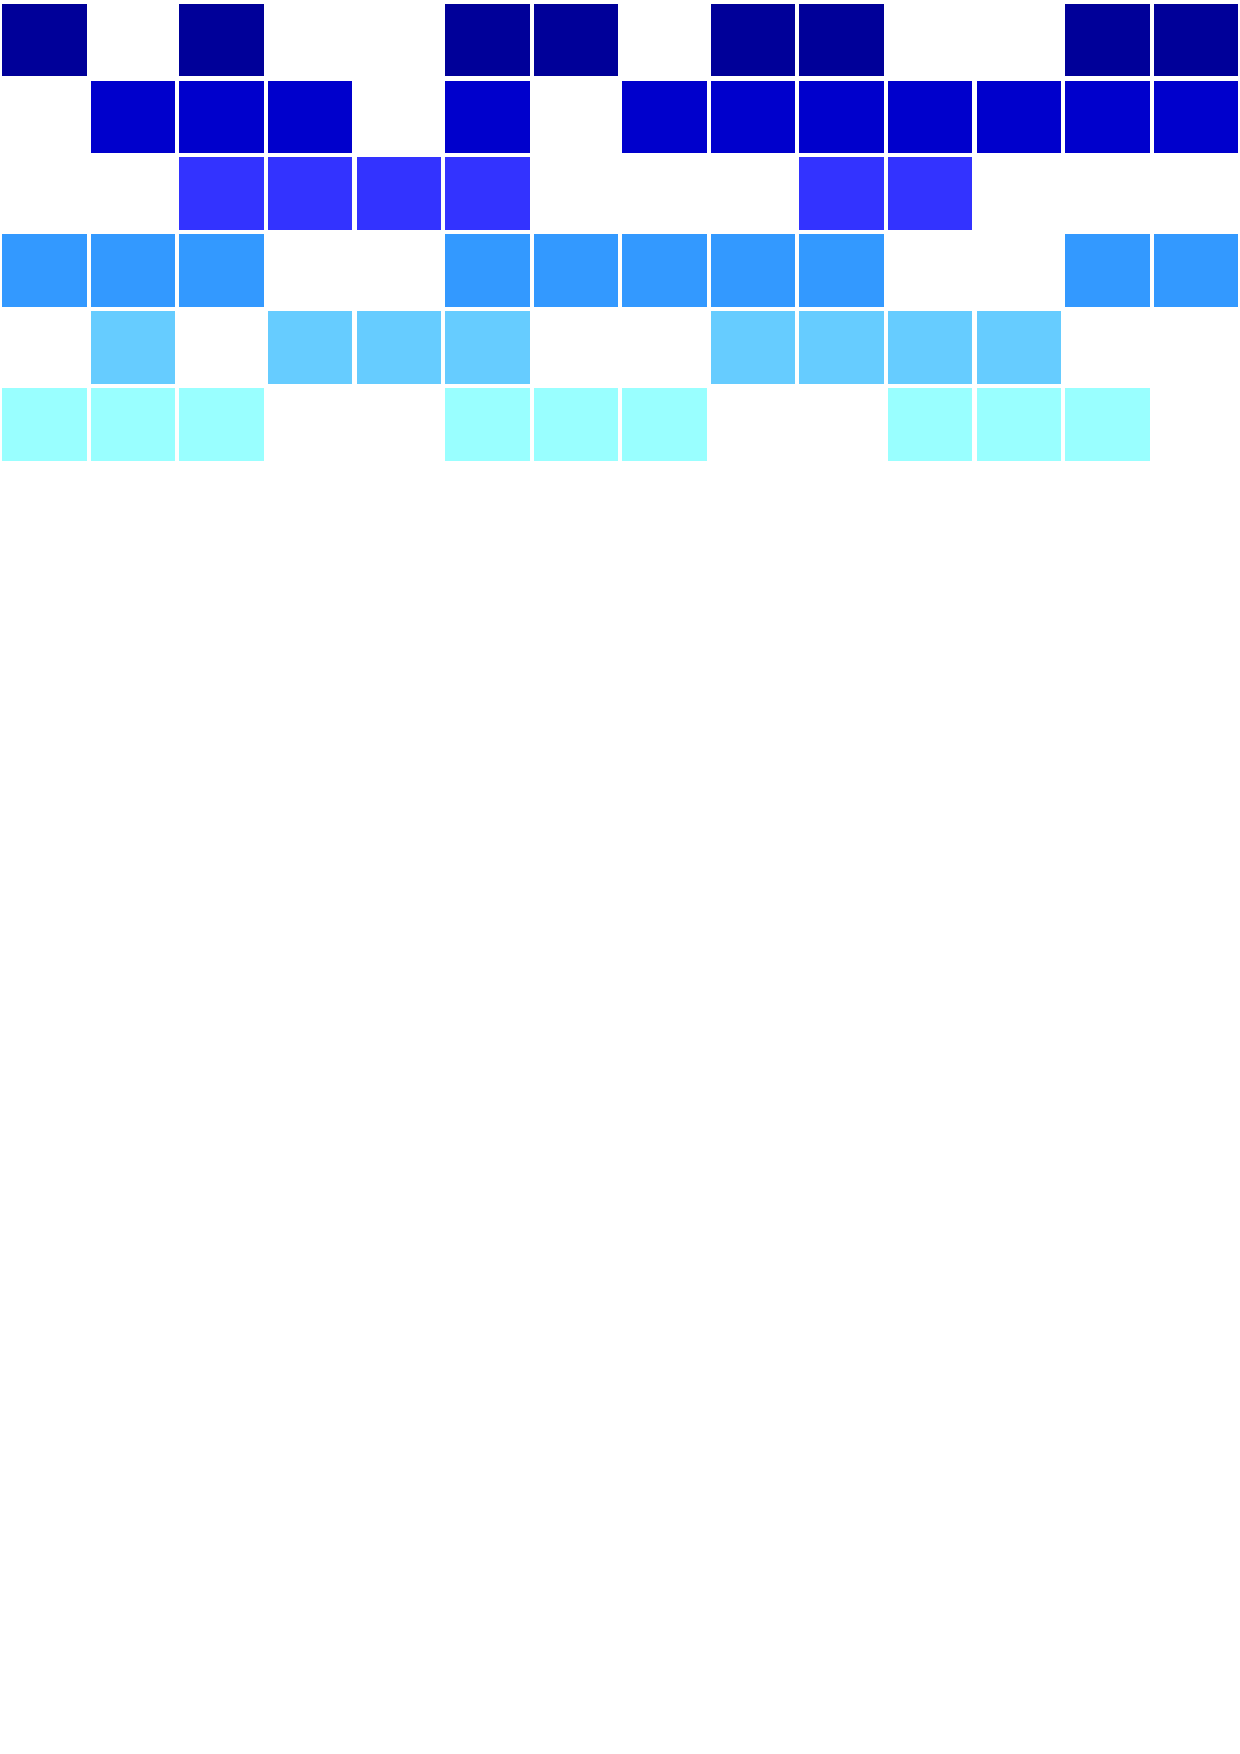
\includegraphics[width=\paperwidth]{background}}; % Background image
\draw[anchor=north] (midpoint) node [fill=ocre!30!white,fill opacity=0.6,text opacity=1,inner sep=1cm]{\Huge\centering\bfseries\sffamily\parbox[c][][t]{\paperwidth}{\centering Circuitos Elétricos\\[15pt] % Book title
{\Large Notas de Aula}\\[20pt] % Subtitle
{\huge Bruno de Araujo Coutinho}}}; % Author name
\end{tikzpicture}};
\end{tikzpicture}
\vfill
\endgroup


%----------------------------------------------------------------------------------------
%	TABLE OF CONTENTS
%----------------------------------------------------------------------------------------

%\usechapterimagefalse % If you don't want to include a chapter image, use this to toggle images off - it can be enabled later with \usechapterimagetrue

\chapterimage{chapter_head_1.pdf} % Table of contents heading image

\pagestyle{empty} % No headers

\tableofcontents % Print the table of contents itself

\cleardoublepage % Forces the first chapter to start on an odd page so it's on the right

\pagestyle{fancy} % Print headers again

%----------------------------------------------------------------------------------------
%	CHAPTER 1: Conceitos Básicos
%----------------------------------------------------------------------------------------
\chapterimage{chapter_head_2.pdf} % Chapter heading image
\chapter{Conceitos Básicos em Circuitos Elétricos}\index{Conceitos Básicos em Circuitos Elétricos}

\section{Engenharia Elétrica: Uma Visão Geral}

O \textbf{engenheiro eletricista} é o profissional que se preocupa com sistemas que produzem, transmitem e medem sinais elétricos. As cinco principais classificações de sistemas elétricos são:
\begin{itemize}
 \item \textbf{Sistemas de Comunicação:} são sistemas elétricos que geram, transmitem e distribuem informações.
 \item \textbf{Sistemas de Computação:} usam sinais elétricos para processar informações, desde palavras até cálculos matemáticos.
 \item \textbf{Sistemas de Controle:} usam sinais elétricos para regular processos, como temperaturas, pressões e escoamento em uma indústria química.
 \item \textbf{Sistemas de Potência:} geram e distribuem energia elétrica. A energia elétrica é gerada por geradores nucleares, elétricos ou térmicos e distribuída por uma rede de condutores.
 \item \textbf{Sistemas de Processamento de Sinais:} agem sobre sinais elétricos que representam informação. Eles transformam os sinais e a informação neles contidas em uma forma mais adequada.
\end{itemize}

\begin{definition}[Circuito Elétrico]
Um \textbf{circuito elétrico} é um modelo matemático que sem comporta aproximadamente como um sistema elétrico real.
\end{definition}

Três premissas nos permitem utilizar a teoria de circuitos para estudar um sistema físico representado por um circuito elétrico:
\begin{enumerate}
 \item Efeitos elétricos acontecem instantaneamente em todo o sistema;
 \item A carga líquida em cada componente do sistema é sempre zero;
 \item Não há nenhum acoplamento magnético entre os componentes de um sistema.
\end{enumerate}

A seguir temos alguns procedimentos gerais para a resolução de problemas:
\begin{enumerate}
 \item Identifique o que é dado e o que tem que ser encontrado;
 \item Desenhe um diagrama do circuito ou outro modelo visual;
 \item Consulte vários métodos de solução e decida pelo que parece mais apropriado para a situação;
 \item Encontre uma solução;
 \item Teste sua solução.
\end{enumerate}

\section{Unidades do Sistema}

O \textbf{Sistema Internacional de Unidade (SI)} habilita os engenheiros a comunicarem resultados quantitativos; As unidades básicas do SI são baseadas em sete quantidades: comprimento (metro - m), massa (quilograma - kg), tempo (segundo - s), corrente elétrica (ampère - A), temperatura termodinâmica (kelvin - K), quantidade de matéria (mol) e intensidade luminosa (candela - cd). Algumas unidades derivadas do SI são: frequência (hertz - $s^{-1}$), foça (newton (N) - $kg \cdot m/s^{2}$).

\section{Análise de Circuito: Uma Visão Geral}

\begin{figure}[h]
\centering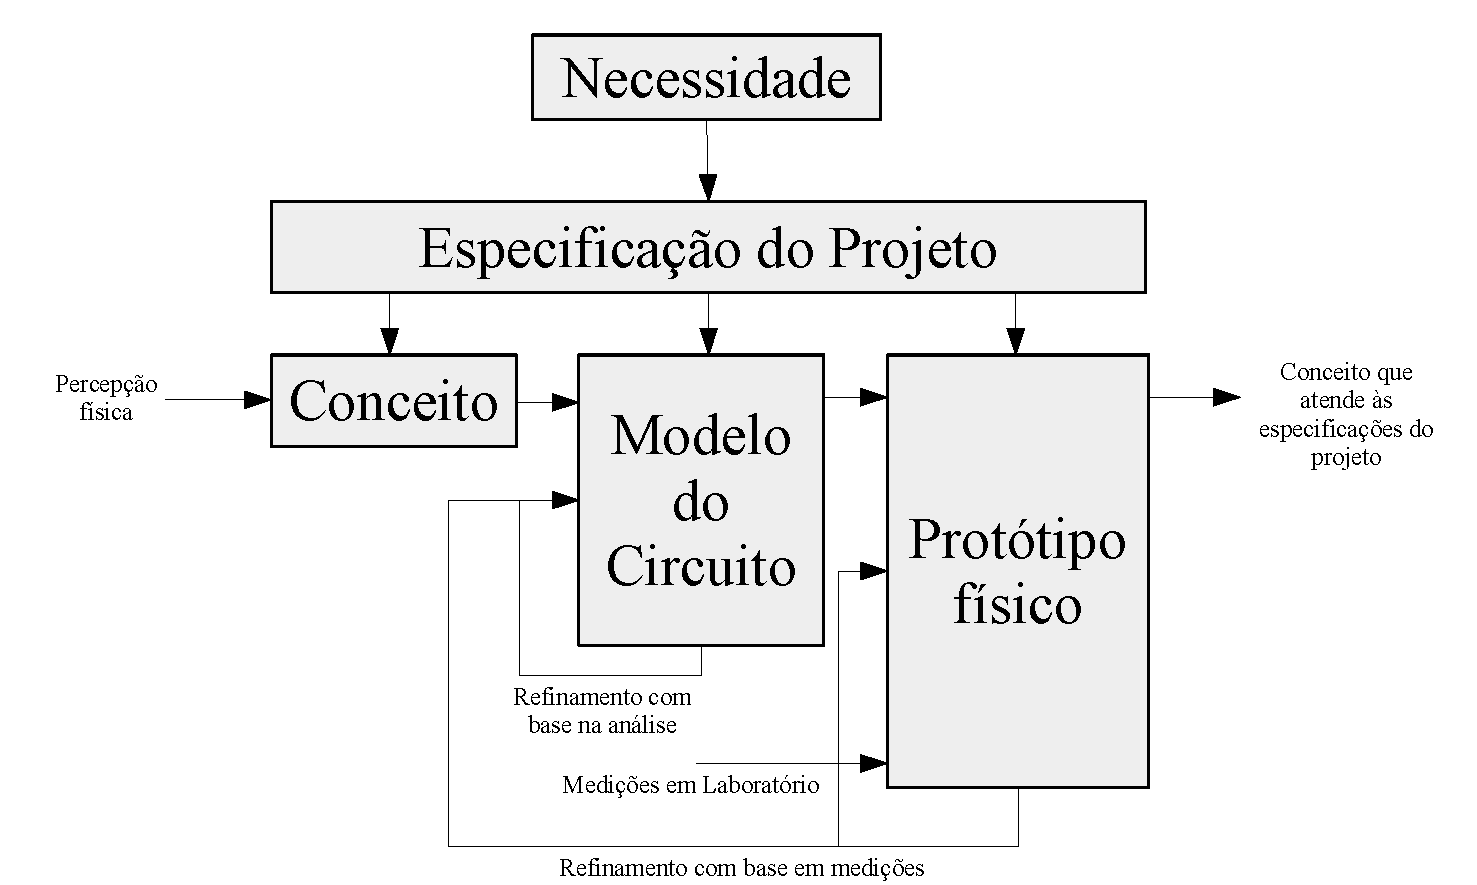
\includegraphics[scale=0.5]{analise_visao_geral}
\caption{Visão Geral da Análise de Circuitos}
\end{figure}

\section{Tensão e Corrente}

Características da carga elétrica:
\begin{enumerate}
\item A carga elétrica é bipolar, o que significa que efeitos elétricos são descritos em termos de cargas negativas e positivas.
\item A carga eletrica existe em quantidades discretas, que são múltiplos inteiros da carga eletrônica, $1.6022 \times 10^{-19}$.
\item Efeitos elétricos são atribuídos tanto à separação entre cargas, quanto a cargas em movimento.
\end{enumerate}

Na teoria de circuitos, a separação entre cargas dá origem a uma força elétrica (tensão), e seu movimento dá origem a um fluxo elétrico (corrente). A análise de circuitos é baseada nestas duas variáveis.

A análise de circuitos é baseada nas variáveis tensão e corrente.

\begin{definition}[Tensão]
 Tensão é a energia por unidade de carga criada pela separação entre cargas. Sua unidade é o \textit{volt}. Expressamos essa razão em forma de diferencial:
\begin{equation}
v = \frac{d w}{dt}
\end{equation}
onde v é tensão em volt (V), w é a energia em joule (J) e q é a carga em coulomb (C).
\end{definition}

\begin{definition}[Corrente]
 Corrente é a taxa de fluxo de carga em movimento em relação ao tempo. Sua unidade é o \textit{ampére}. Expressamos essa razão em forma de diferencial:
\begin{equation}
i = \frac{d q}{dt}
\end{equation}
onde i é a corrente em ampére (A), q é a carga em coulomb (C) e t é o tempo em segundo (s).
\end{definition}

\section{Elemento Básico Ideal de Circuito}

O \textbf{elemento básico ideal de cirucuito} é um componente com dois terminais que não pode ser subdividido; ele pode ser descrito matematicamente em termos da tensão e da corrente em seus terminais.

\begin{figure}[h]
\centering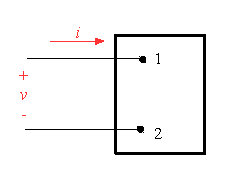
\includegraphics[scale=1]{elemento_basico_ideal}
\caption{Elemento Ideal de Circuito}
\end{figure}

A \textbf{convenção passiva} usa um sinal positivo na expressão que relaciona a tensão e a corrente nos terminais de um elemento quando a direção de referência  para a corrente que passa pelo elemento está na direção da queda de tensão de referência no elemento.

\begin{exercise}
 A corrente nos termiais de um elemento é dada por:
 \[
 \begin{cases}
  i = 0 & t < 0 \\
  i = 20e^{-5000t} & t \ge 0
 \end{cases}
 \]
 Calcule a carga total (em microcoulombs) que entra em seu terminal.
\end{exercise}

\begin{exercise}
 A expressão para a carga que entra no terminal superior de um elemento ideal de circuito é
 \[
	q = \frac{1}{\alpha^2} - ( \frac{t}{\alpha} + \frac{1}{\alpha^2} )e^{-\alpha t} [C]
 \]
 Determine o valor máximo da corrente elétrica que entra no terminal se $\alpha = 0.03679 s^{-1}$
\end{exercise}

\section{Potência e Energia}

\begin{definition}[Potência]
 Potência é a taxa de variação temporal do gasto ou da absorção de energia. É a energia por unidade de tempo e é igual ao produto da tensão e da corrente nos terminais. Sua unidade no SI é o watt (W).
 \begin{equation}
  p = \frac{d w}{dt}
 \end{equation}
\end{definition}

A potência decorrente do fluxo de carga vem da definição:

$$ p = \frac{d w}{dt} = \frac{d w}{dq} \cdot \frac{d q}{dt} = v \cdot i $$

\begin{equation}
 p = v \cdot i
\end{equation}

%----------------------------------------------------------------------------------------
%	CHAPTER 2: Elementos de Circuitos
%----------------------------------------------------------------------------------------
\chapter{Elementos de Circuitos}

\section{Fontes de Tensão e de Corrente}

Uma fonte elétrica é um dispositivo capaz de converter energia não elétrica em energia elétrica. Uma fonte ideal de tensão é um elemento de circuito que mantém uma tensão prescrita em seus terminais independentemente da corrente que flui sobre eles. Uma fonte ideal de corrente mantém uma corrente prescrita em seus terminais independentemente da tensão sobre eles.

Uma fonte independente estabelece

\section{Resistência Elétrica}

\begin{definition}[Resistência]
Resistência é a capacidade dos materiais de impedir o fluxo de corrente ou, mais especificamente, o fluxo de carga elétrica. O elemento de circuito usado para modelar esse comportamento é o \textbf{resistor}.
 \begin{circuitikz} \draw
  (0,0) to[R, l=$R$] (2,0); 
 \end{circuitikz}
\end{definition}

Para fins de análise de circuitos, devemos referir à corrente no resistor à tensão terminal. A relção entre a tensão e a corrente em um resistor é:

\begin{equation}
 v = i R
 \label{leiohm}
\end{equation}

Esta equação é conhecida como \textbf{Lei de Ohm}.

\section{Leis de Kirchhoff}

Diz-se que um circuito está resolvido quando a tensão nos terminais de cada elemento e a corrente correspondente foram determinadas.

Circuitos são descritos por nós e caminhos fechados. Um \textbf{nó} é um ponto no qual dois ou mais elementos de circuito se unem.

%----------------------------------------------------------------------------------------
%	CHAPTER 3: Circuitos Resistivos Simples
%----------------------------------------------------------------------------------------
\chapter{Circuitos Resistivos Simples}

\section{Resistores em Série}

Elementos de circuito ligados em série conduzem a mesma corrente.

\section{Resistores em Paralelo}

Elementos de circuito ligados em paralelo têm a mesma tensão em seus terminais

\section{Circuitos Divisores de Tensão e de Corrente}

\section{Medição de Corrente e de Tensão}

\section{Medição de Resistência}

\section{$\Delta$-Y}

%----------------------------------------------------------------------------------------
%	CHAPTER 4: Técnicas de Análise de Circuitos
%----------------------------------------------------------------------------------------
\chapter{Técnicas de Análise de Circuitos}

\section{Terminologia}

\section{Método das Tensões de Nó}

%----------------------------------------------------------------------------------------
%	CHAPTER 7: Análise da Potência CA
%----------------------------------------------------------------------------------------
\chapter{Análise da Potência CA}

\section{Potência instantânea e potência média}

A \textbf{potência instantânea}, $p(t)$, em watts, é a taxa na qual um elemento absorve energia. É a potência a qualquer instante.

\begin{equation}
 p(t) = v(t) \cdot i(t)
\end{equation}

Considerando $v(t) = V_m cos(\omega t + \theta_v)$ e $i(t) = I_m cos(\omega t + \theta_i)$ e aplicando uma identidade trigonométrica \footnote{$cos(A)cos(B) = \frac{1}{2}cos(A-B) + \frac{1}{2}cos(A+B)$}, podemos expressar a potência como:

\begin{equation} \label{potinst}
 p(t) = \frac{1}{2}V_m I_m \cos(\theta_v - \theta_i) + \cos(2 \omega t + \theta_v + \theta_i)
\end{equation}

\begin{tikzpicture}
\begin{axis}[axis lines = left, xlabel = t (s), ylabel = V]
\addplot[domain=0:360,samples=100,color=red]{sin(x)};
\end{axis}
\end{tikzpicture}

A \textbf{potência média}, em watts, é a média da potência instantânea ao longo de um período.

\begin{equation}
 P = \frac{1}{2} \int_0^T p(t) dt
\end{equation}

Para a expressão na Equação \ref{potinst}, temos que:

\begin{equation}
 P = \frac{1}{2} V_m I_m cos(\theta_v - \theta_i)
\end{equation}

<demonstração>

Note que $p(t)$ cvaria com o tempo, ao passo que $P$ não.

As formas fasoriais de $v(t)$ e $i(t)$  são, respectivamente, $\mathbf{V} = V_m \angle \theta_v$ e $\mathbf{I} = I_m \angle \theta_i$. Para usar fasores, percebemos que:

\begin{align}
 \frac{1}{2} \mathbf{V}\mathbf{I^*} &= \frac{1}{2} = V_m I_m \angle \theta_v - \theta_i \\
 &= \frac{1}{2} V_m I_m [\cos(\theta_v - \theta_i) + j \sin(\theta_v - \theta_i)]
\end{align}

Reconhecemos a parte real dessa expressão como a potência média, P.

Em um circuito resistivo, $\theta_v = \theta_i$, então, $\cos(\theta_v - \theta_i) = 1$, nos dando

\begin{equation}
 P = \frac{1}{2} V_m I_m = \frac{1}{2} {I_m}^2 R
\end{equation}

Quando $\theta_v - \theta_i = +- 90^{\circ}$, temos que $\cos(\theta_v - \theta_i) = 0$. Então, em um circuito putamente reativo, a potência média é zero.

<3 exemplos>

\section{Transferência de Potência média Máxima}

Considere o equivalente de Thévenin de um circuito:

<figura>

Na morma retangular, as impedâncias são:

\begin{align}
 Z_{Th} &= R_{Th} + j X_{Th} \\
 Z_L &= R_L + j X_L
\end{align}

A corrente através da carga será:

\begin{equation}
 \mathbf{I} = \frac{\mathbf{V}_{Th}}{Z_{Th} + Z_L} = \frac{\mathbf{V}_{Th}}{(R_{Th} + R_L) + j (X_{Th} + X_L)}
\end{equation}

A potência média na carga então será

\begin{equation} \label{potencia}
 P = \frac{1}{2} |\mathbf{I}|^2 \cdot R_L = \frac{|\mathbf{V}_{Th}| R_L / 2}{(R_{Th} + R_L)^2 + (X_{Th} + X_L)^2}
\end{equation}

Tomando $\partial P / \partial R_L$ e $\partial P / \partial X_L$ e igualando ambas expressões a zero, vamos ter:

%\begin{align}
% X_L &= - X_{Th} \label \\
% R_L &= \sqrt{{R_{Th}}^2 + (X_{Th} + X_L)^2}
%\end{align}

Combinando as Equações, conclui-se que para haver a máxima transferência,

\begin{equation}
 Z_L = {Z_{Th}}^{*}
\end{equation}

Fazendo $Z_L = {Z_{Th}}^{*}$ na Equação \eqref{potencia}, vamos obter a potência média máxima na carga:

\begin{equation}
 P_{\text{máx}} = \frac{|\mathbf{V}_{Th}|^2}{8 R_{Th}} 
\end{equation}

<exemplos>

\section{Valor Eficaz ou RMS}

\textbf{Valor eficaz} de uma corrente periódica é a corrente

%----------------------------------------------------------------------------------------
%	BIBLIOGRAPHY
%----------------------------------------------------------------------------------------

\chapter*{Bibliography}
\addcontentsline{toc}{chapter}{\textcolor{ocre}{Bibliography}}
\section*{Books}
\addcontentsline{toc}{section}{Books}
\printbibliography[heading=bibempty,type=book]
\section*{Articles}
\addcontentsline{toc}{section}{Articles}
\printbibliography[heading=bibempty,type=article]

%----------------------------------------------------------------------------------------
%	INDEX
%----------------------------------------------------------------------------------------

\cleardoublepage
\phantomsection
\setlength{\columnsep}{0.75cm}
\addcontentsline{toc}{chapter}{\textcolor{ocre}{Index}}
\printindex

%----------------------------------------------------------------------------------------

\end{document}
